\documentclass{article}
\usepackage[margin=1in]{geometry}

\usepackage{graphicx}
\usepackage{amsmath}
\usepackage{amssymb} % \gtrsim is defined here
%\usepackage[colorlinks=true, allcolors=blue]{hyperref} % for \url
\usepackage{hyperref}
\begin{document}
\part{Normalized clustering coefficients}


\section{Introduction}

\subsection{Current measures for clustering}

Local clustering coefficient \cite{Watts1998}:

\begin{equation} \label{eq:Cws}
    c_i = 
    \left\{
    	\begin{array}{ll}
    		\dfrac{2 T_i}{k_i (k_i-1)}  & \mbox{if } k_i > 1 \\
    		0 & \mbox{if } k_i \leq 1,
    	\end{array}
    \right.
\end{equation}

where $T_i$ is the number of triangles passing through vertex $i$ and $k_i$ is its degree.

Average Watts-Strogatz clustering coefficient:
\begin{equation}
    \bar{c} = \dfrac{1}{N} \sum_i c_i.
\end{equation}

Obs: This average is taken over all the nodes in the network. Some authors use, instead, the only the nodes with degree greater than 1. It is important to be aware of that when interpreting results of other authors.

Degree-dependent clustering coefficient \cite{Vazquez2002Large-scaleInternet}:

\begin{equation}
    \bar{c}(k) = \dfrac{1}{N_k} \sum_{i\in Y(k)} c_i = \dfrac{1}{k(k-1)N_k} \sum_{i\in Y(k)} 2T_i,
\end{equation}

where $N_k$ is the number of nodes with degree $k$ and $Y(k)$ is the set of such nodes.

The quantities $\bar{C}$ and $\bar{c}(k)$ are related by

\begin{equation}
    \bar{c} = \sum_k p(k) \bar{c}(k),
\end{equation}

$p(k)$ being the degree distribution.

A different global transitivity measure $C$ was introduced by Newman in \cite{Newman2003}, and is defined as 

\begin{equation} \label{eq:C}
    C = \dfrac{2T}{\sum_i k_i (k_i-1)},
\end{equation}

where $T = \sum_i T_i$ is the number of triangles in the network.

The two global clustering coefficients have similar definitions and, in fact, for some networks both have similar values. In particular, for an uncorrelated network, $\bar{C}$, $\bar{c}(k)$ and $C$ are identical and its value can be computed as \cite{NewmanBook} 

\begin{equation} \label{eq:Cunc}
C_{\mathrm{unc}} = \dfrac{1}{N} \dfrac{\left[ \langle k^2 \rangle - \langle k \rangle  \right]^2}{\langle k \rangle^3}.
\end{equation}

Nevertheless, these coefficients do differ significantly in some cases, as can be seen in \cite{Bollobs2004, Estrada2011}. Usually, Equation \ref{eq:Cws} gives larger values than Equation \ref{eq:C} (see, for example, \cite{NewmanBook}, footnote, p. 334).

\subsection{Normalized clustering coefficient}

We define the normalized clustering coefficients

\begin{equation} \label{eq:Cnorm}
C_{\mathrm{norm}} = \dfrac{C - C_{\mathrm{rand}}}{C_{\mathrm{max}} - C_{\mathrm{rand}}}\qquad \text{and} \qquad
\bar{c}_{\mathrm{norm}} = \dfrac{\bar{c} - \bar{c}_{\mathrm{rand}}}{\bar{c}_{\mathrm{max}} - \bar{c}_{\mathrm{rand}}}
\end{equation}

$C_{\mathrm{rand}}$ and $\bar{c}_{\mathrm{rand}}$ represent the average of the clustering coefficient computed for an ensemble of random networks with the same degree sequence as the original network, and $C_{\mathrm{max}}$ and $\bar{c}_{\mathrm{max}}$ correspond to the maximum clustering values that can be achieved over the networks in the ensemble. In our work, we will consider the ensamble of all networks having the same degree sequence as the original network.

There are differen posibilities in which $C_{\mathrm{rand}}$ can be defined. One way is using the expected value for an uncorrelated network, given by Equation \ref{eq:Cunc}, which can be easily computing from the degree sequence. Unfortunately, this measure has some problems for heterogeneous graphs (for which the hypothesis of no degree-degree correlations is not satisfied), as is exemplified in Appendix \ref{app:Cunc}. The alternative is to create instances of randomized versions of the network and define $C_{\mathrm{rand}}$ as the average of the clustering coefficient for a set of such instances. In this line, we used two different randomization procedures. The first one is the Configuration Model \cite{Molloy1995ASequence}, and the second method consists in randomizing the original network by degree-preserving edge rewiring. %The two randomization approaches are similar, but not exactly the same. One of the main differences is that when the network is dense ($\langle k \rangle \gtrsim 10$)

The Configuration Model is an algorithm that allows to build a network with a given degree sequence from scratch. It works as follows. We start with an empty graph with $N$ nodes (being $N$ the size of the desired network). We then attach to each node a number of ``half-edges'' or stubs equal to the node's degree. Then, with uniform probability we pick a pair of stubs and join them, forming an edge. We repeat this step until there is no more free stubs. The algorithm does not impose any restriction on the graph connectivity, and can even create double-edges and self-loops. If one is interested in generating simple graphs, there are two options. The first is to repeatedly apply the algorithm until the resulting graph is simple. It has been proved [TODO: add reference] that by doing that, the sampling is uniform among all the simple graph with the given degree sequence. The downside of this alternative is that it can be computationally prohibitive, in particular for networks with diverging $\langle k^2 \rangle$, where the probability sampling a simple graph is very low \cite{NewmanBook}. The second alternative is to remove all the self-loops and double-edges from the sampled graph. The expected number of such edges is $\frac{1}{2} \left[ (\langle k^2 \rangle - \langle k \rangle ) / \langle k \rangle \right]^2$ \cite{NewmanBook}, so it vanishes for $N\rightarrow \infty$ as long as $\langle k^2 \rangle$ remains bounded. This means that this second alternative is practical for networks that are not too heterogeneous. In this work, we chose this second alternative, for which we created 100 random graphs and then took the average of the corresponding clustering coefficients.

The method of degree-preserving edge rewiring (also known as edge swapping or markov chain approach) has been widely used in the literature \cite{Orsini2015QuantifyingNetworks} [TODO: add more references]. It consists on randomly selecting a pair of non-adjacent edges and, if no double edge is created in the process, swapping them. This procedure preserves the degree sequence, but destroys degree correlations. It has been shown that a number $\gtrsim M$ of swaps is enough to decorrelate the network. Here, we performed 10 independent realizations with a total of $n = 100 M$ swaps for networks small networks ($M < 100000$) and  $n = 10 M$ swaps for big networks ($M < 100000$) [TODO: add references related to mixing time and ergodicity for edge swapping]. 

\subsection{Maximum clustering coefficient}

The definitions given by equation \ref{eq:Cnorm} require the knowledge of the greatest value for the clustering coefficient that can be achieved by a graph having a specified degree sequence. In this section we will address how to compute that value.

\subsubsection{Approximation of $C_{\mathrm{max}}$} \label{sec:intro_Cmax}

{\bf Havel-Hakimi algorithm:}

This is a known algorithm that is very useful because it allows to determine whether a given degree sequence is graphic or not \cite{Hakimi1962}. It is based on the Havel-Hakimi theorem, which states that the degree sequence $S = [k_1, k_2, ..., k_N]$, where $k_i \geq k_j,\; \forall i\leq j$, is graphic if and only if the sequence $S' = [k_2-1, k_3-1, ..., k_{k_1+1}-1, k_{k_1+2} ,..., k_N]$ is also graphic. If the given list $S$ is graphic, then the theorem will be applied at most $N-1$ times setting in each further step $S:=S'$. Note that it can be necessary to sort this list again. This process ends when the whole list $S'$ consists of zeros. In each step of the algorithm one constructs the edges of a graph with vertices $v_1, ..., v_N$, i.e. if it is possible to reduce the list $S$ to $S'$, then we add edges $\lbrace v_1, v_2 \rbrace, \lbrace v_1, v_3 \rbrace, \lbrace v_1, v_{d_1+1} \rbrace,$. When the list $S$ cannot be reduced to a list $S'$ of non-negative integers in any step of this approach, the theorem proves that the list $S$ from the beginning is not graphic.

The advantage of this algorithm is that it always converges when the original sequence is graphic and that the resulting graph es quite clusterized. The disadvantage is that in general it doesn't give the most clusterized graph. For example, given the degree sequence $S_1 = [3, 3, 2, 2, 2, 1, 1]$, the result of the algorithm is the graph in left side of figure \ref{fig:graph_3322211}, whilst the most clustered graph for that degree sequence is the graph in the right part of the figure.

\begin{figure}[ht!]
\centering
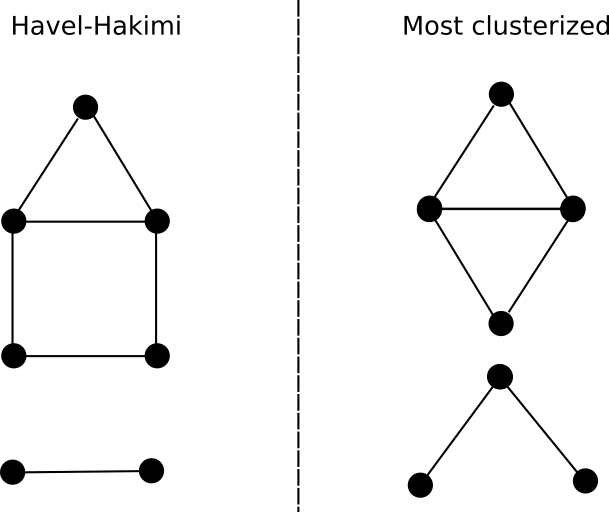
\includegraphics[scale=0.7]{./figs/graph_3322211.png}\hfill%
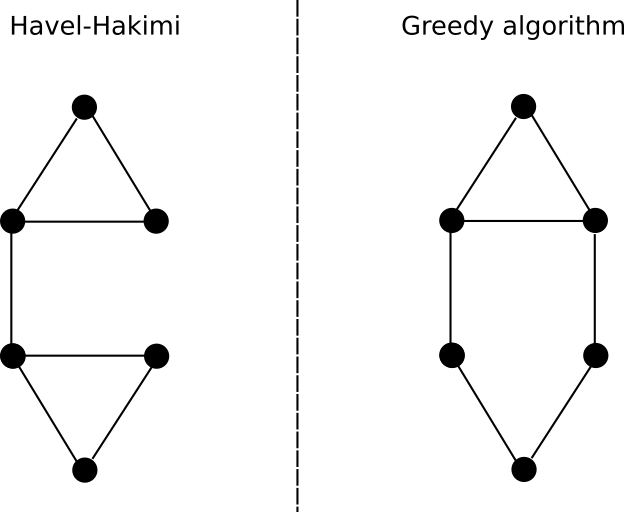
\includegraphics[scale=0.7]{./figs/graph_332222.png}
\caption{(Left) Graphs obtained from the degree sequence $S_1 = [3, 3, 2, 2, 2, 1, 1]$. (Right) Graphs obtained from the degree sequence $S_1 = [3, 3, 2, 2, 2, 2]$.}
\label{fig:clusteredGraphExamples}
\end{figure}

{\bf Greedy algorithm:}

This algorithm is similar as the Havel-Hakimi algorithm, with the difference that at each step the list is not sorted. This algorithm gives very good results for most of the real-world networks we studied (the resulting graph is more clusterized than the graph using the Havel-Hakimi algorithm). In particular, in the example in figure \ref{fig:fig:clusteredGraphExamples} (left), it finds the most clusterized graph. Also, comparing with Monte Carlo simulations, it seems that this algorithm finds graphs with a clustering coefficient very close to the maximum. 

The main disadvantage of this algorithm is that it doesn't always converge. One counterexample is the degree sequence $S_2 = [3, 3, 2, 2, 2, 2]$ (Figure \ref{fig:clusteredGraphExamples} right). After adding the edges $\lbrace v_1, v_2 \rbrace$, $\lbrace v_1, v_3 \rbrace$, $\lbrace v_1, v_4 \rbrace$, $\lbrace v_2, v_3 \rbrace$, $\lbrace v_2, v_4 \rbrace$,$ \lbrace v_5, v_6 \rbrace$, the algorithm is stuck, as there is no possible pair of nodes where to put the last edge. To overcome this flaw, we  perform the following modification. Whenever the algorithm get stuck, lets say after adding the edge $\lbrace v_i, v_j \rbrace$, we remove this edge and try to connect node $v_i$ with $v_{j+1}$. If the algorithm stuck after adding the edge $\lbrace v_i, v_N \rbrace$, we try with $\lbrace v_{i+1}, v_j \rbrace$. This way, the algorithm always converges. 

In most cases, this algorithm seems to converge to graphs very close to the most clustered graph. But if we see the example $S_2$, we can show that the result of the algorithm is the graph in the right side of figure.

{\bf Monte Carlo approach}

The third approach for finding the most clusterized graph with a given degree sequence is by performing a degree preserving rewiring process which attempts to increase the number of triangles at each step. This procedure is similar to the one described in \cite{Tamm2014IslandsNetworks} and consists in a standard Monte Carlo process using the Metropolis algorithm. We consider the ensemble of all networks having a specified degree sequence. Each triangle in the network is weighted with a chemical potential $\mu$. The partition function of the ensemble is 

\begin{equation}
Z(G, \mu) = \sum e^{\mu N_T},
\end{equation}

where $N_T$ is the number of triangles of the network $G$ and the sum runs over all networks having the same degree sequence. The MC algorithm consists on a set of degree-preserving rewiring steps. After each rewiring attempt is performed, if the number of triangles increases, the step is accepted. If the number of triangles decreases in a number $\Delta N_T$, it is accepted with probability $e^{-\mu \Delta N_T}$.

The protocol is the following: we start with $t_0 M$ rewiring steps performed at $\mu = 0$ to randomize the network (here $M$ is the number of links). Then, the chemical potential is increased by an amount $\Delta \mu$ and $t_1 M$ steps are performed to reach equilibrium. After that, we take $n_s$ samples of the system, with a space between sample of $t_2 M$ steps, and compute the relevant quantities (for example, the clustering coeficients). When the chemical potential reaches the value $\mu_{\mathrm{max}}$, we change $\Delta \mu$ by $-\Delta \mu$ and compute the reverse process up to $\mu = 0$.


\section{Results}

\subsection{$C_{\mathrm{max}}$ for real-world networks}

In Figure \ref{fig:Cmax_MC_and_greedy}, we show the Monte Carlo calculations for different real-world netowrks, together with the value for the Newman clustering coefficient obtained by using the greedy algorithm described in Section \ref{sec:intro_Cmax}. As it can be seen, the MC process finds configurations with greater values than the greedy algorithm, thus the latter does not give the most clusterized graph. For most networks, the differences are not significant, and the greedy algorithm be used as a good approximation. Some networks, nonetheless, exhibit an important difference between these two values.

In Figure \ref{fig:Cmax_MC_vs_greedy} we show the two quantities. It can be seen that most points lay near the diagonal, but there are some outliers.

\begin{figure}[ht!]
\centering
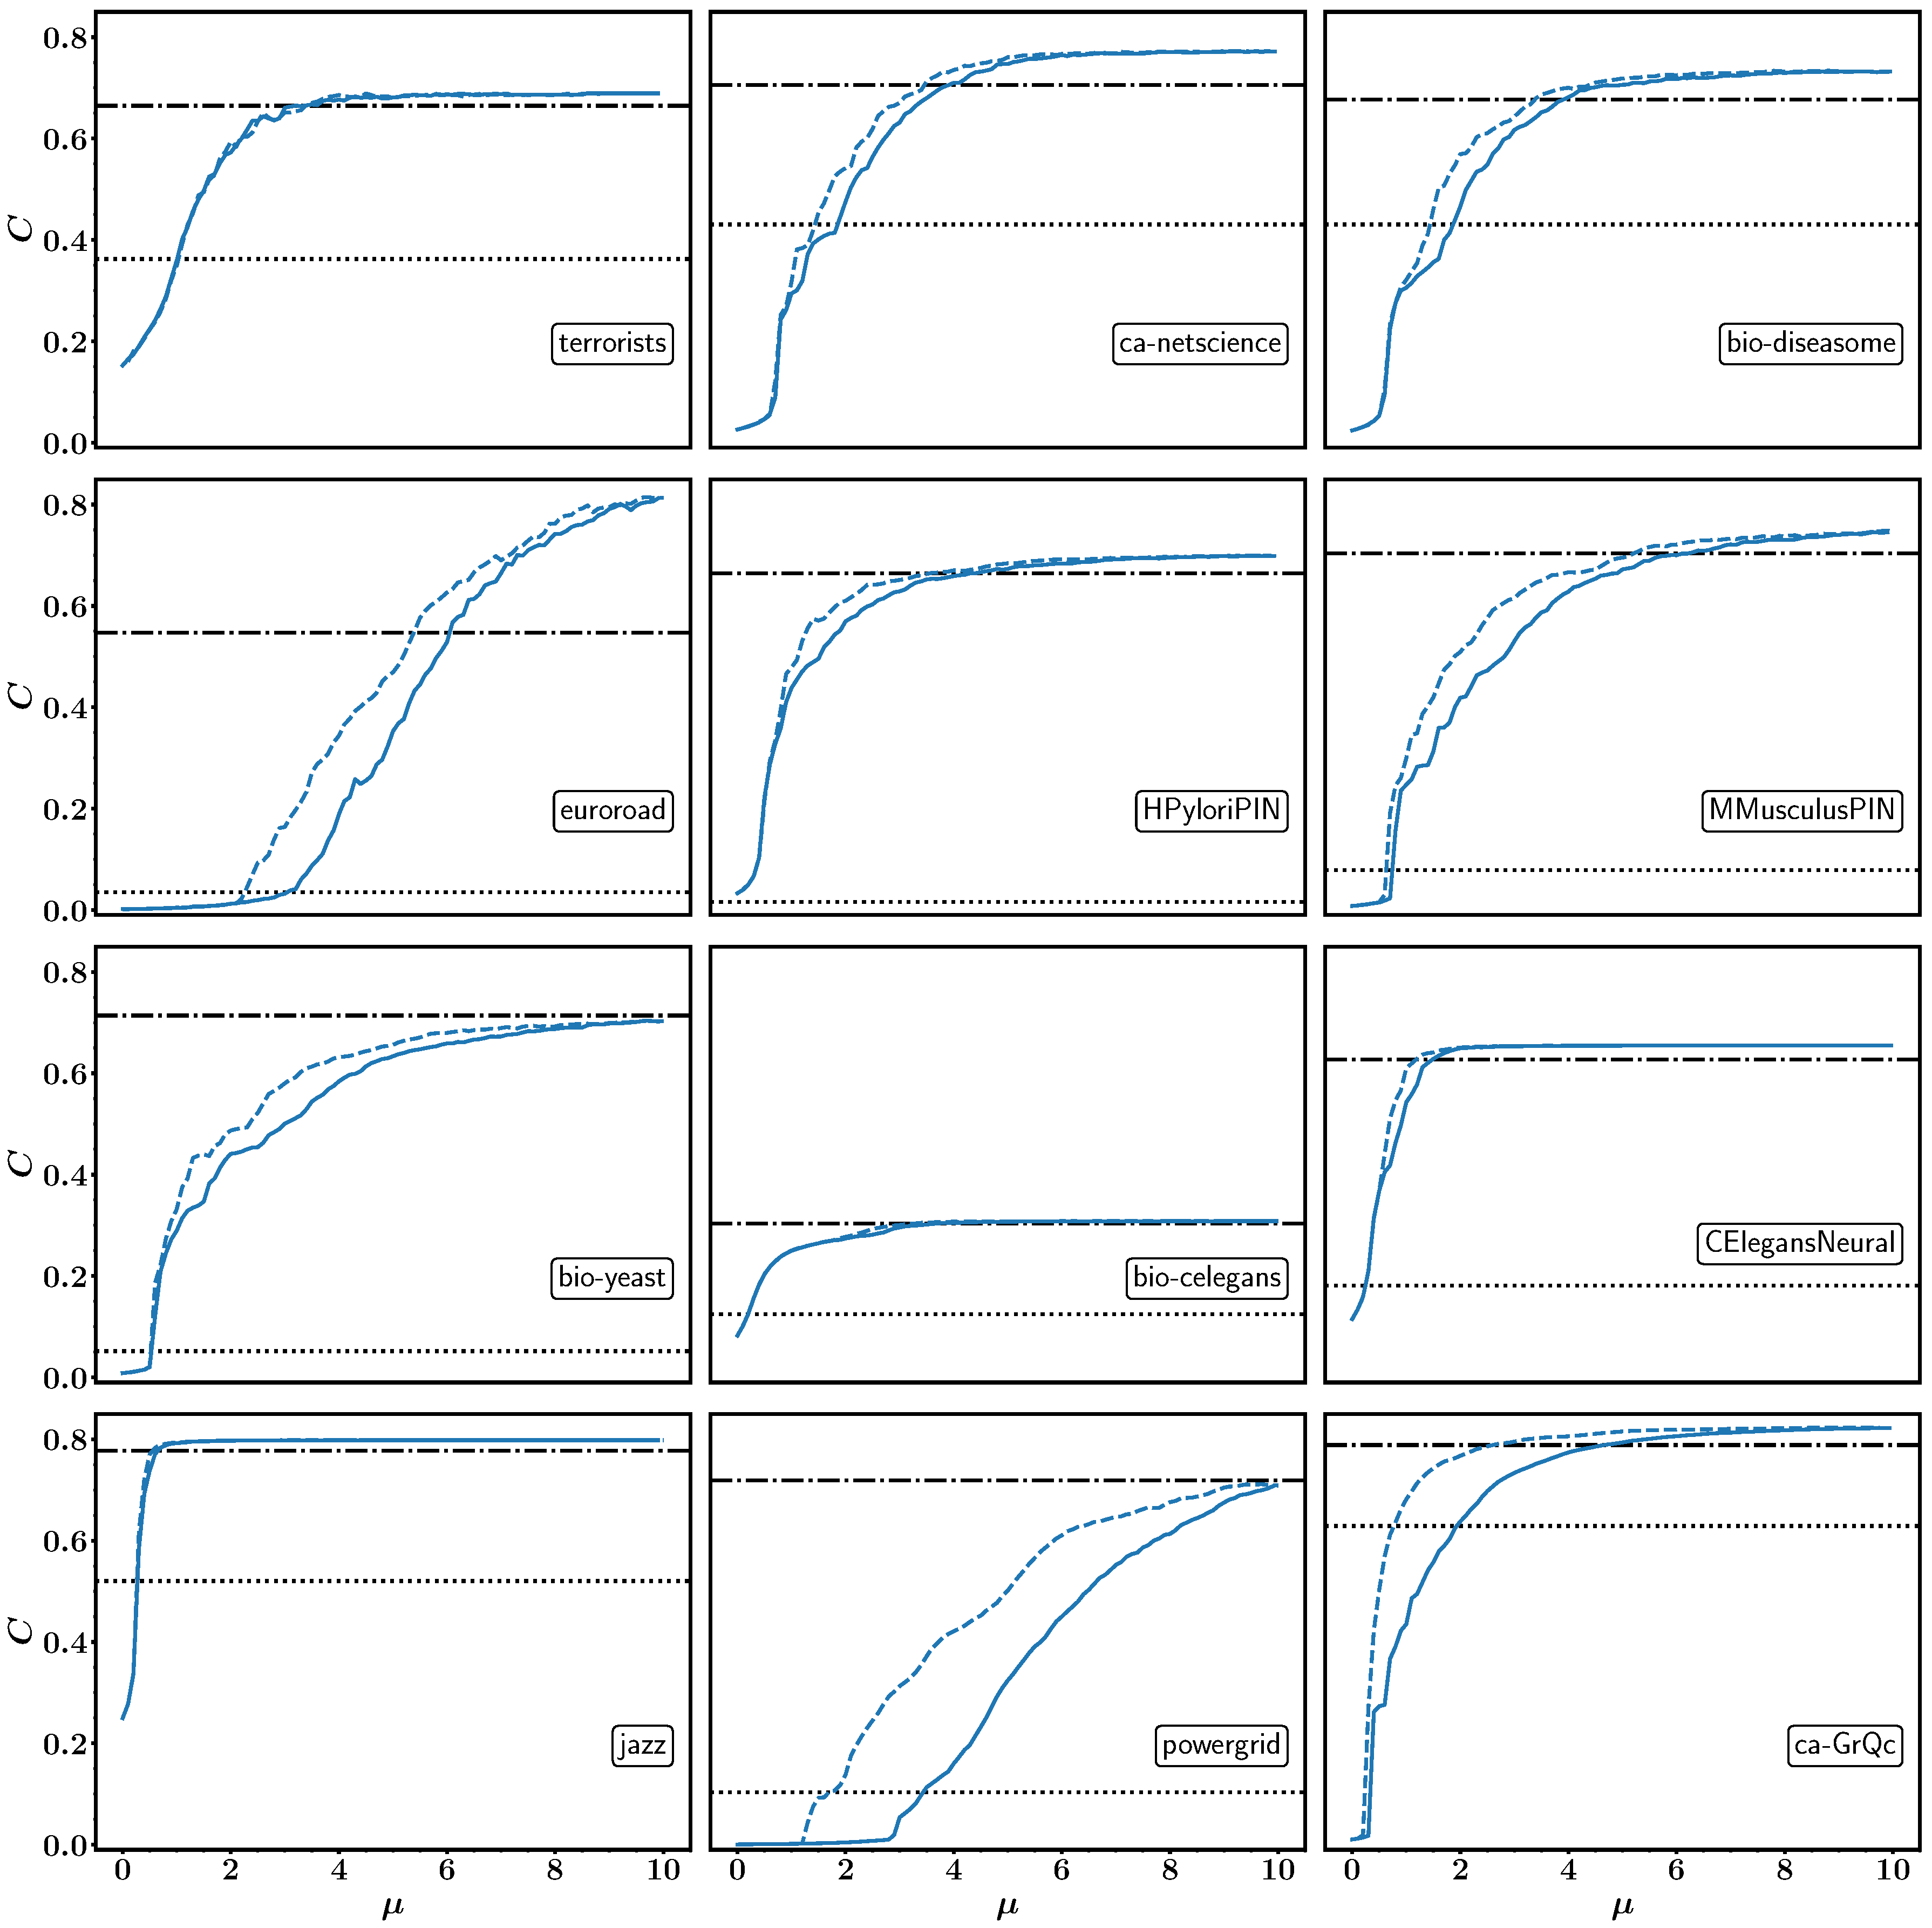
\includegraphics[scale=0.26]{./figs/Cmax_MC_and_greedy}
\caption{Variation in the clustering coefficient using the Monte Carlo process for incrementing the number of triangles in different real-world networks. Solid blue lines correspond to the diraction of increasing $\mu$ and dashed blue lines to decreasing values. The horizontal dotted line is the clustering coefficient for the original network and the horizontal dotted-dashed line, the value obtained using the greedy algorithm. The parameters for the Monte Carlo calculations are $\Delta \mu = 0.1$, $t_0 = 100$, $t_1 = 100$, $t_2 = 10$ and $n_s = 100$.}
\label{fig:Cmax_MC_and_greedy}
\end{figure}

\begin{figure}[ht!]
\centering
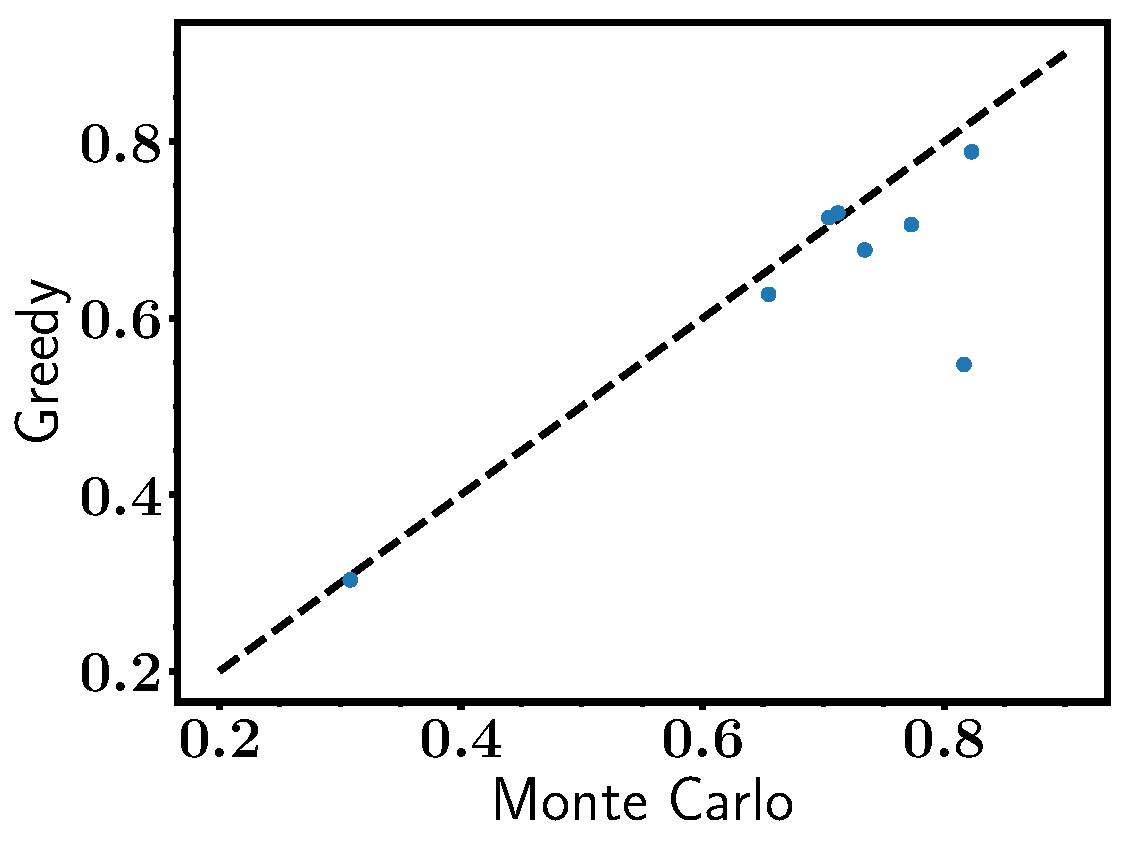
\includegraphics[scale=0.35]{./figs/Cmax_MC_vs_greedy}
\caption{Differences between the maximum value of the clustering coefficient $C$ obtained by the greedy algorithm and the Monte Carlo process.}
\label{fig:Cmax_MC_vs_greedy}
\end{figure}

\subsection{Normalized clustering coefficient for real-world networks}

The normalized clustering coefficient was computed for several real-world networks (a full list of the networks studied, together with a description of each one) is provided in Appendix \ref{app:NetworksStudied}. In Figure \ref{fig:Cnorm_vs_C} we show the normalized version of the Newman clustering coefficient.

\begin{figure}[ht!]
\centering
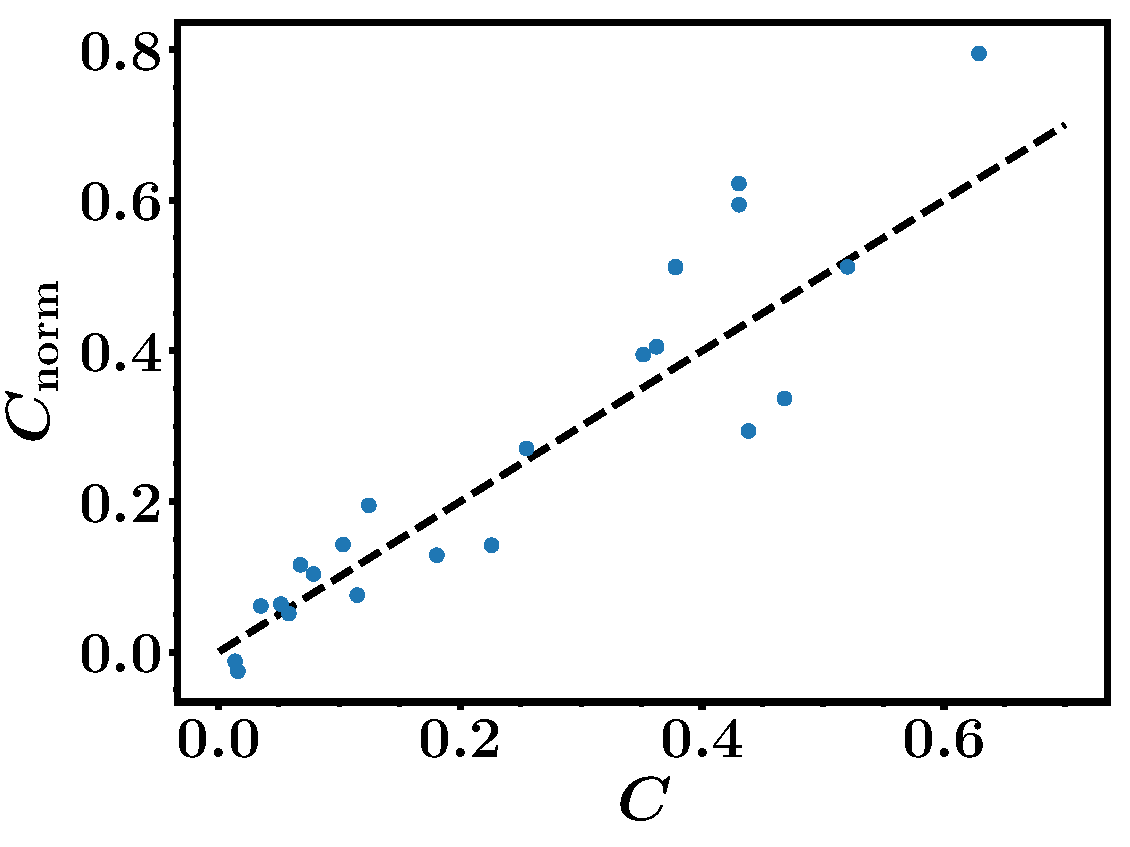
\includegraphics[scale=0.4]{./figs/Cnorm_vs_C}
\caption{Normalized clustering coefficient compared with its standard version. In this case, $C_{\mathrm{max}}$ was computed using the greedy algorithm and $C_{\mathrm{rand}}$ using the configuration model.}
\label{fig:Cnorm_vs_C}
\end{figure}

\appendix
\section{Problems with $C_{\mathrm{unc}}$} \label{app:Cunc}

Equation \ref{eq:Cunc} is valid under the condition that no degree-degree correlation exist. In graphs with an heterogeneous degree distribution, such correlations are unavoidable, and this expresion could give incorrect values. For details, see ref. \cite{Newman2003WhyNetworks}.

Lets consider a few examples. Suppose we have a star graph with $N+1$ nodes. This graph has one single node with degree $N$ and $N$ nodes with degree $1$. the first and second momenta of the degree distribution are 

\begin{align}
    \langle k \rangle &= \dfrac{1}{N+1} \sum_{i=0}^N k_i = \dfrac{1\times N + N \times 1}{N+1} = \dfrac{2N}{N+1} \nonumber \\
    \langle k^2 \rangle &= \dfrac{1}{N+1} \sum_{i=0}^N k_i^2 = \dfrac{1\times N^2 + N \times 1^2}{N+1} = \dfrac{N^2 + N}{N+1} = N
\end{align}

If we apply equation \ref{eq:Cunc} to this particular case, we obtain

\begin{equation}
    C_{\mathrm{unc}} = \dfrac{1}{N+1}\dfrac{\left(N^2-\dfrac{2N}{N+1} \right)^2}{\left(\dfrac{2N}{N+1} \right)^3}= \dfrac{\left[N^2(N+1)-2N\right]^2}{(2N)^3} = \dfrac{(N^3+N^2-2N)^2}{8N^3},
\end{equation}

which is an increasing function of $N$ and is greater than 1 for $N \geq 3$.
\\

Now suppose we have a sparse network (with mean degree independent of $N$) and with degree distribution with second momentum scaling as $\langle k^2 \rangle \sim N^{\alpha}$, with $\alpha > 0$. In this case, equation \ref{eq:Cunc} gives

\begin{equation}
    C_{\mathrm{unc}} \sim N^{2\alpha},
\end{equation}

which is unbounded for $\alpha > 0$. That means that the expression for the expected clustering coefficient in uncorrelated networks is not valid for networks that are too heterogeneous. 

Now, lets consider the case in which we have a very connected hub with degree $k_{\mathrm{max}} \sim N^{\alpha}$. Suppose also that the degree of the rest of the nodes doesn't scale with $N$. In this case, we have, for $N\gg 1$, 

\begin{align}
    \langle k \rangle &\sim N^{\alpha - 1} \nonumber \\
    \langle k^2 \rangle &\sim N^{2\alpha-1} \nonumber 
\end{align}

Then, equation \ref{eq:Cunc} gives 

\begin{equation}
    C_{\mathrm{unc}} \sim \dfrac{1}{N} \dfrac{(N^{2\alpha-1} - N^{\alpha - 1})^2}{N^{3(\alpha - 1})} \sim \dfrac{N^{4\alpha-2}}{N^{3\alpha-2}} \sim N^{\alpha}.
\end{equation}

Thus, if the hub scales with $N$ with any positive exponent, the expected clustering coefficient diverges.

\section{Computing $C_{\mathrm{rand}}$}

In this section, we will discuss the differences betweenn using the Configuration Model and the rewiring procedure to compute $C_{\mathrm{rand}}$.

In Figure \ref{fig:relaxation}, we show how the clustering coefficients vary as the network is relaxed to an uncorrelated version using the rewiring procedure. As it can be seen, in most networks a number of iterations equal to $M$ is enough to fully randomize it. 

\begin{figure}[ht!]
\centering
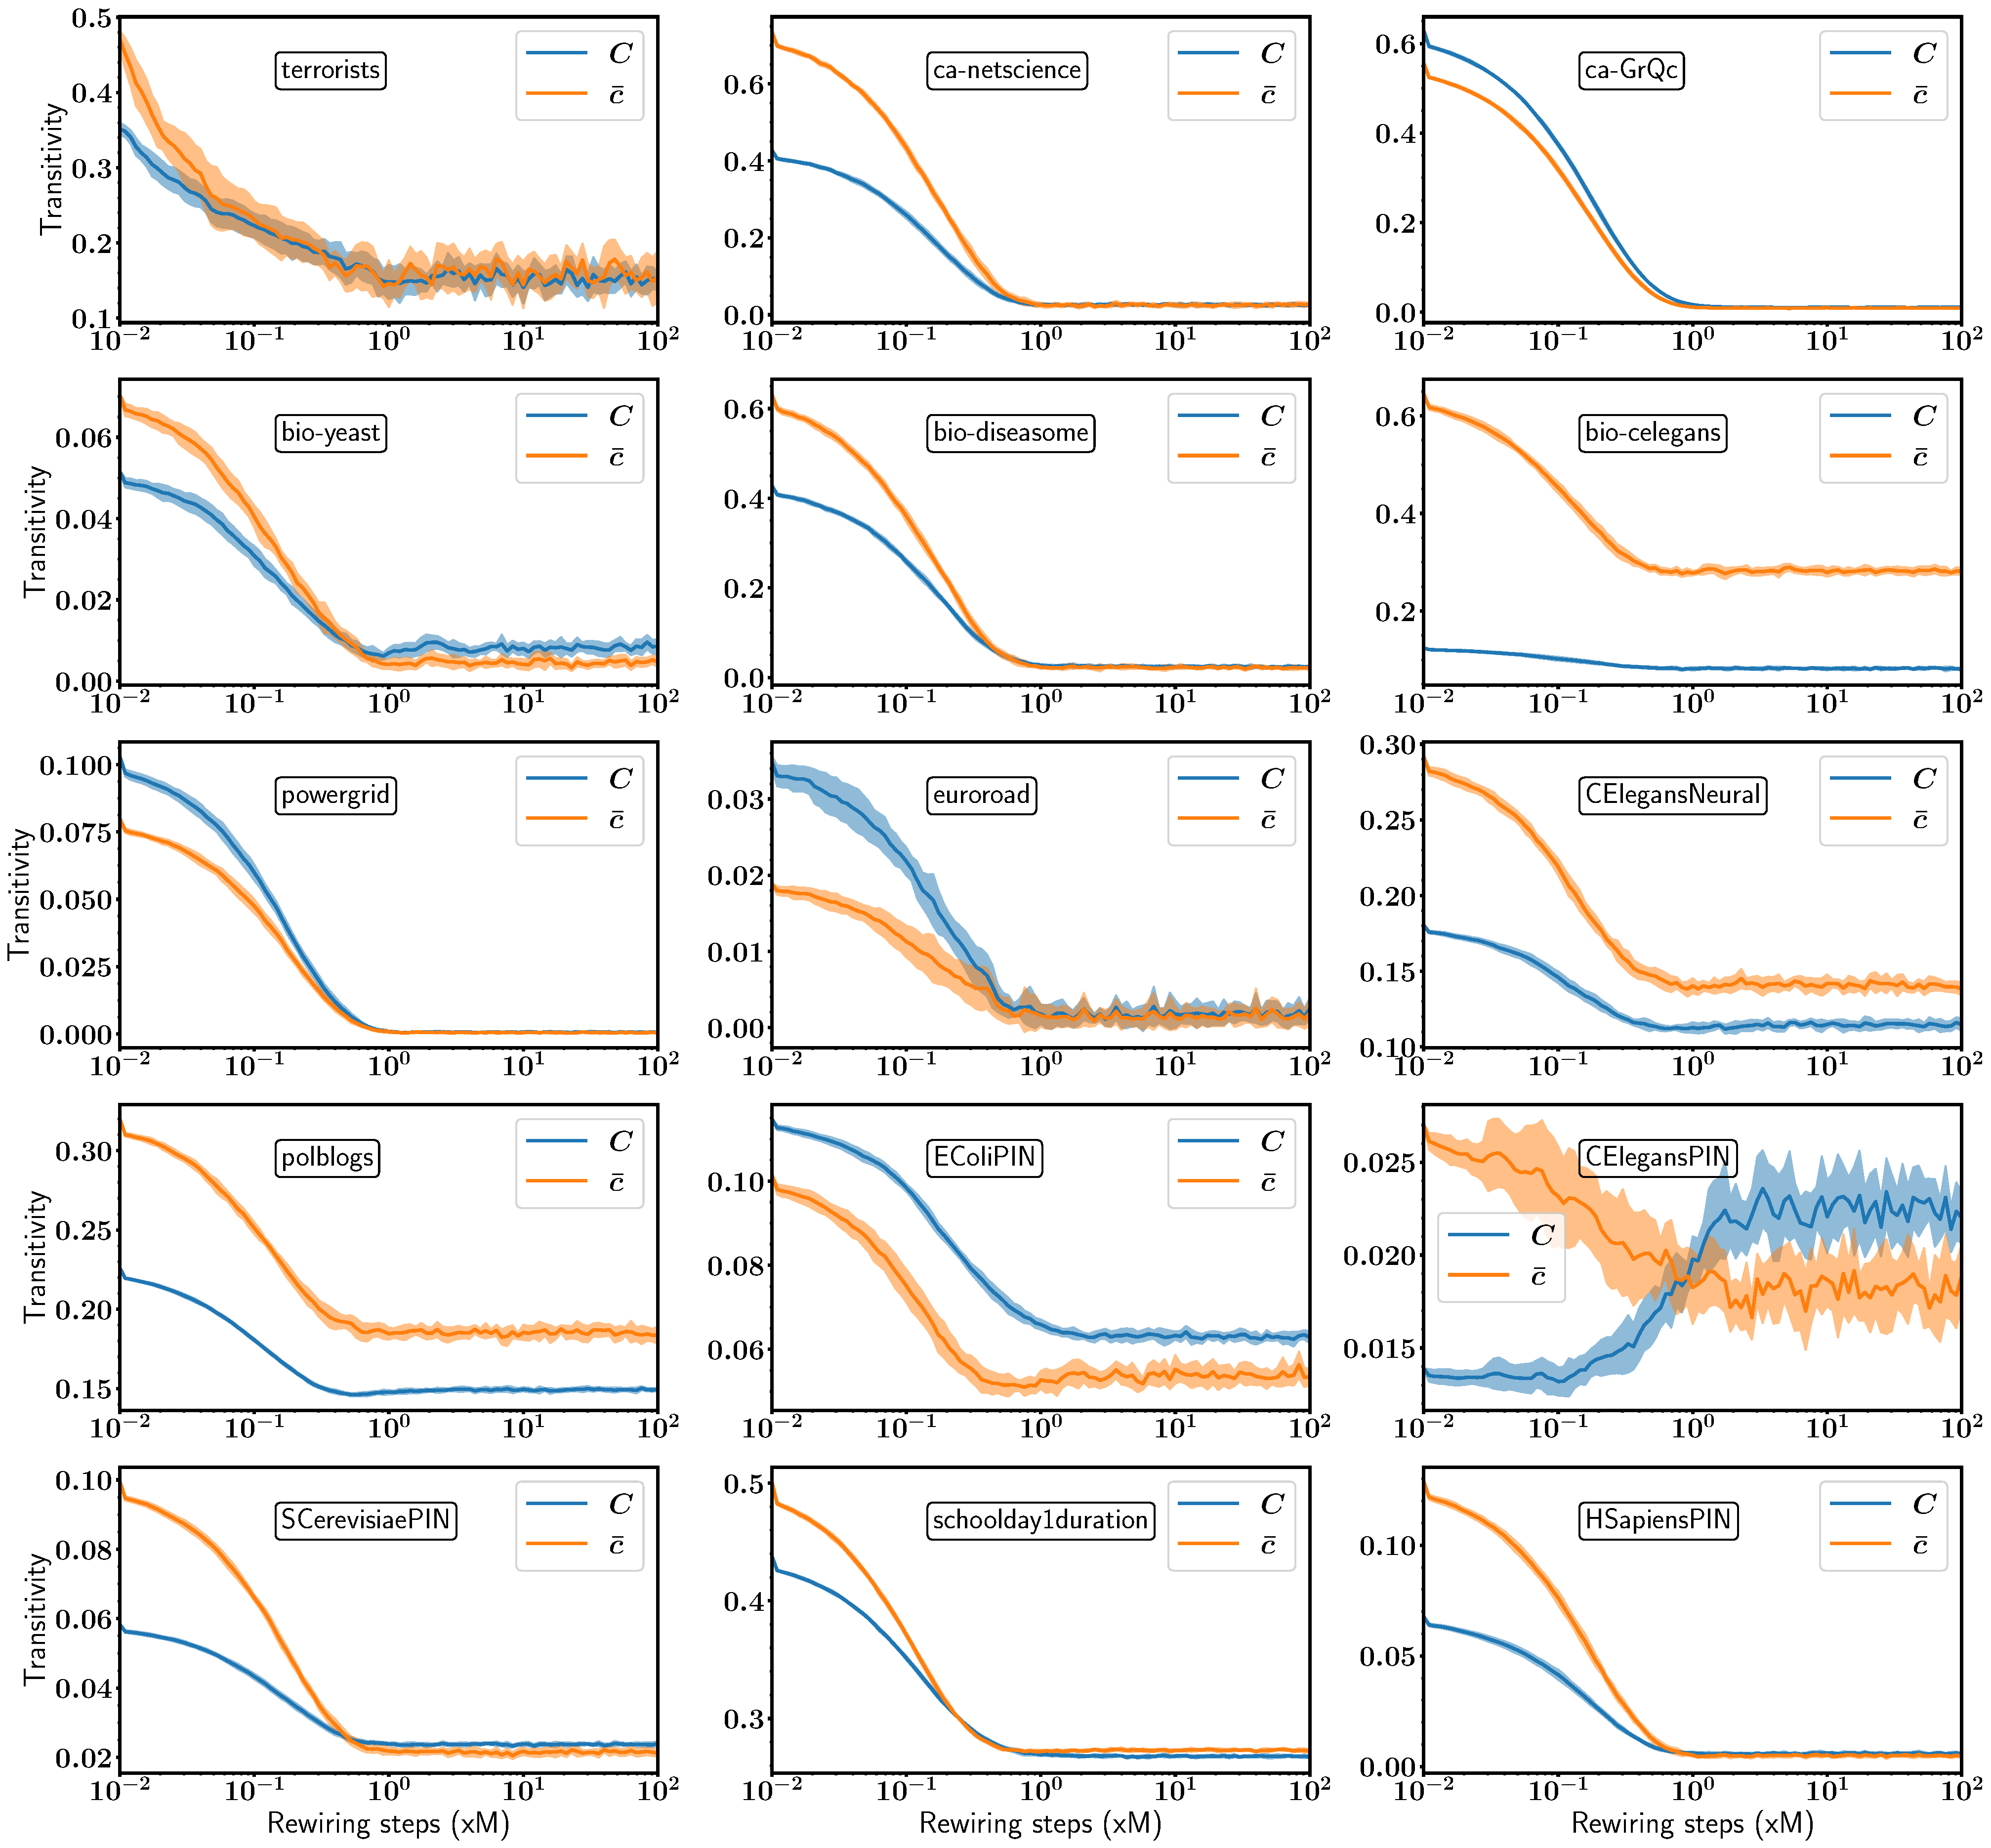
\includegraphics[scale=0.26]{./figs/relaxation.pdf}
\caption{Relaxation of different real-world networks using the rewiring procedure. After $\sim M$ rewiring steps, the network converges to its random version. Each curve correspond to an average taken over $10$ realizations, and shade regions correspond to a standard deviation from the mean.}
\label{fig:relaxation}
\end{figure}

Whilst the rewiring procedure keeps the degree sequence fixed, the configuration model can in principle produce multiple edges, as well as self loops. Given that the clustering coefficients are defined for simple graphs, if that happens, it is necesary to simplify the graph before computing the values. Once simplified, the resulting graph will have a different degree sequence than the original, so the values of the clustering coefficients computing using this null model could potentially differ from the values obtained by the rewiring process. As it is pointed out in \cite{NewmanBook}, the expected number of multiple edges can be computed as

\begin{equation}
\text{Expected number of multiple edges} = \dfrac{1}{2}  \left( \dfrac{\langle k^2 \rangle - \langle k \rangle}{\langle k \rangle}\right)^2,
\end{equation}

 so as long as the two first momenta of the degree distribution remains bounded, the fraction of multiple edges vanishes as $1/N$ and the degree sequence generated by the configuration model is asymptotically the same as the original graph. In Figure \ref{fig:CrandCM_vs_CrandRewire} we show that indeed, the differences between these two values are not significant.

\begin{figure}[ht!]
\centering
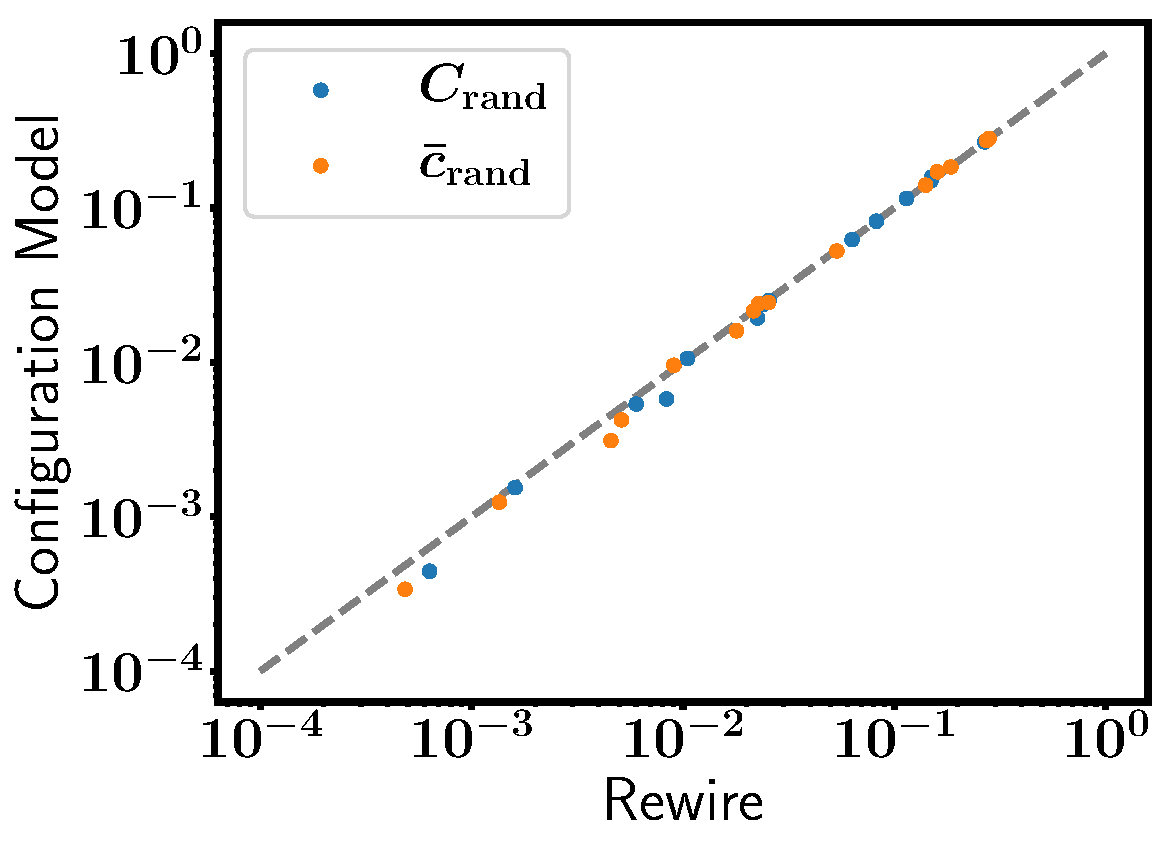
\includegraphics[scale=0.35]{./figs/CrandCM_vs_CrandRewire.pdf}
\caption{Comparison between the transitivity values obtained in the two null models proposed: configuration model and rewiring process.}
\label{fig:CrandCM_vs_CrandRewire}
\end{figure}

\section{Analytic Results}

In this Appendix we will discuss the problem of finding the maximum value of the clustering coefficient for a given degree sequence.

In \cite{Rivin2002}, Rivin obtains sharp bounds for the number of $n$-cycles in a simple, undirected graph as a function of the number of edges. In particular, the bound for the number $T$ of triangles of a network with $N$ nodes and $M$ edges is found. Using Lagrange multipliers to maximize 

\begin{equation}
    \sum_i \lambda_i^3
\end{equation}

under the constraints

\begin{equation}
    \sum_i \lambda_i = 0\qquad \text{and} \qquad \sum_i \lambda_i^2,
\end{equation}

he obtains that the number of triangles is bounded by

\begin{equation} \label{eq:RivinBound}
    T \leq \dfrac{N-2}{\sqrt{N (N-1)}} \dfrac{2^{1/2}}{3} M^{3/2}.
\end{equation}

Also, taking the complete graph as an example, he proves that the bound is sharp.

Now, inequality \ref{eq:RivinBound} could be improved by imposing the condition that the network has a specified degree sequence.

Let G be a simple undirected graph with $N$ nodes and $M$ links and let $A$ be its adjacency matrix. The elements $a_{ij}=(A)_{ij}$ then satisfy

\begin{align}
    a_{ij} &= a_{ji}, \\
    a_{ii} &= 0, \\
    \sum_{j} a_{ij} &= k_i, \\
    \sum_{i, j} a_{ij} &= 2M,
\end{align}

where $k_i$ is the degree of the node $i$.
\\

%where $\lbrace k_1, k_2, \dots, k_N\rbrace$. L
The Newman's clustering coefficient is given by

\begin{equation}
    C = \dfrac{6 \times N_T}{|P_2|} 
\end{equation}

where $N_T$ is the number of triangles in the network and $|P_2|$ the number of path of length 2.

To compute the number of path of length two, lets start by noting that, for a given node $i$, the number of path of length 2 that start in $i$ are

\begin{equation}
    |P_2|(i) = \sum_{l} (A^2)_{il} - (A^2)_{ii}=  \sum_{lj} a_{il} a_{lj} - k_i = \sum_{l} a_{il} k_l - k_i.
\end{equation}

Then, the total number of paths of length two is simple 

\begin{equation} \label{eq:P2}
    %|P_2| = \sum_i |P_2|(i) = \sum_i \sum_{l\neq j} a_{il} a_{lj} = \sum_{ilj} a_{il} a_{lj} - k_i = \sum_l k_i^2 - 2M
    |P_2| = \sum_i |P_2|(i) = \sum_i \left( \sum_{l} a_{il} k_l - k_i \right) = \sum_l k_l^2 - 2M.
\end{equation}

On the other side, the number of triangles in the graph is given by

\begin{equation} \label{eq:T}
    %N_T = \dfrac{1}{6} Tr(A^3) = \dfrac{1}{6} \sum_{i} c_{ii} = \dfrac{1}{6} \sum_{ijl} a_{ij} a_{jl} a_{li}
    N_T = \dfrac{1}{6} Tr(A^3) = \dfrac{1}{6} \sum_{ijl} a_{ij} a_{jl} a_{li}.
\end{equation}

Thus, the Newman's clustering coefficient is given by

\begin{equation} \label{eq:newman}
    C = \dfrac{Tr(A^3)}{|P_2|} = \dfrac{Tr(A^3)}{\sum_l k_l^2 - 2M},
\end{equation}

If we consider the ensamble of graphs having a given degree sequence $\lbrace k_1, k_2, \dots, k_N\rbrace$, the clustering coefficient depends only on the numerator of equation \ref{eq:newman}, as the denominator is determined by the degree sequence.

The Watts-Strogatz clustering coefficient is defined by

\begin{equation} \label{eq:ws}
    C_{\mathrm{WS}} = \dfrac{1}{N} \sum_{i} c(i),
\end{equation}

where $c(i)$ is the local clustering of node $i$, defined as

\begin{equation}
    c(i) = 
    \left\{
    	\begin{array}{ll}
    		\dfrac{2 N_{T}(i)}{k_i (k_i-1)}  & \mbox{if } k_i > 1 \\
    		0 & \mbox{if } k_i \leq 1
    	\end{array}
    \right.
\end{equation}

% \begin{equation}
%     c(i) = \dfrac{2 N_{T}(i)}{k_i (k_i-1)},
% \end{equation}

$N_T(i)$ being the number of triangles that have $i$ as one of its vertices, which can be computed as

\begin{equation}
    N_T(i) = \sum_{jl} a_{ij} a_{jl} a_{li} = (A^3)_{ii}.
\end{equation}

Thus, equation \ref{eq:ws} can be written as

\begin{equation} \label{eq:CwsTheo}
    C_{\mathrm{WS}} = \dfrac{1}{N} \sum\limits_{i:k_i>1}  \dfrac{2 N_{T}(i)}{k_i (k_i-1)} =  \dfrac{1}{N} \sum\limits_{i:k_i>1} \dfrac{2 (A^3)_{ii}}{k_i (k_i-1)} 
\end{equation}


\subsection{Lagrange multipliers}

In order to get $C_{\mathrm{max}}$, we need to maximize the number of triangles in the network (the number of triads is fixed by the degree sequence, see Eq. \ref{eq:P2}). According to Eq. \ref{eq:T}, the number of triangles is determined by the trace of the adjacency matrix A. Considering the degree sequence as constrains, together with the conditions imposed in considering the graph as simple and undirected, the function we have to maximize is

\begin{equation}
    f(\lbrace a_{ij} \rbrace) = Tr(A^3) + \sum_i \theta_i \left(d_i - \sum_j a_{ij} \right) - \sum_i \omega_i a_{ii} + \sum_{i\neq j} \beta_{ij} (a_{ij}-a_{ji}) + \gamma \left(2M - \sum_{ij} a_{ij} \right).
\end{equation}

Differentiating with respect to $a_{ij}$ and equaling to 0,

\begin{equation}
    \dfrac{\partial f(\lbrace a_{pq} \rbrace)}{\partial a_{pq}} = 3 (A^2)_{pq} - \theta_p - \omega_p \delta_{pq} + (\beta_{pq} - \beta_{qp}) (1-\delta_{pq}) - \gamma = 0,
\end{equation}

where $\delta_{pq}$ is the Kronecker delta. For $p=q$, we obtain

\begin{align}
    3 (A^2)_{pp} &= \theta_p + \omega_p + \gamma \\
    3 d_p &=  \theta_p + \omega_p + \gamma.
\end{align}

Summing over $p$,

\begin{equation} \label{eq:diagonal}
    6 M = \Theta + \Omega + N \gamma,
\end{equation}

where we defined $\Theta = \sum_p \theta_p$ and $\Omega = \sum_p \omega_p$.
\\

On the other side, for $p\neq q$, we have

\begin{equation} \label{eq:p_neq_q}
    3 (A^2)_{pq} = \theta_p + (\beta_{qp} - \beta_{pq}) + \gamma.
\end{equation}

Analogously, differentiating with respect to $a_{qp}$, $q \neq p$, we have

\begin{equation}\label{eq:q_neq_p}
    3 (A^2)_{qp} = \theta_q - (\beta_{qp} - \beta_{pq}) + \gamma.
\end{equation}

Taking into account that $A^2$ is symmetric and adding Eq. \ref{eq:q_neq_p} to Eq. \ref{eq:p_neq_q}, 

\begin{equation} \label{eq:A2pnotq}
    6 (A^2)_{pq} = \theta_p + \theta_q + 2 \gamma.
\end{equation} 



Summing \ref{eq:A2pnotq} over $p\neq q$,

\begin{align}
    \sum_{p\neq q}6 (A^2)_{pq} &=\sum_{p\neq q} (\theta_p + \theta_q) +2 N(N-1) \gamma \nonumber \\
    6 |P_2| &= 2(N-1) \Theta + 2N(N-1) \gamma \nonumber \\
    \dfrac{3 |P_2|}{N-1} &= \Theta + N \gamma. \label{eq:sum_mu}
\end{align}

Summing \ref{eq:A2pnotq} over $q:q\neq p$,

\begin{align}
    \sum_{q:q\neq p} (A^2)_{pq} &= (N-1) \theta_p + \sum_{q:q\neq p} \theta_q + 2(N-1)\gamma \nonumber\\ 
    |P_2(p)| &= (N-1) \theta_p + \Theta - \theta_p + 2(N-1)\gamma \nonumber\\ 
    |P_2(p)| &= (N-2) \theta_p + \Theta + 2(N-1)\gamma \nonumber \\
    |P_2(p)| &= (N-2) \theta_p + (N-2)\gamma + \dfrac{3 |P_2|}{N-1} \nonumber \\
    |P_2(p)| &= (N-2) (\theta_p + \gamma) + \dfrac{3 |P_2|}{N-1}
\end{align}

From \ref{eq:diagonal} and \ref{eq:sum_mu}, we have 

\begin{equation}
    \Omega = 6M - \dfrac{3 |P_2|}{N-1}.
\end{equation}



Summing over $p\neq q$,

%Then, the parameters $\mu_p$ satisfy

%\begin{equation}\label{eq:sum_mu}
%    \sum_p \mu_p = \dfrac{3 |P_2|}{N-1}
%\end{equation}

Now, subtracting Eq. \ref{eq:q_neq_p} to Eq. \ref{eq:p_neq_q}, we have

\begin{equation}\label{eq:betas}
     2 (\beta_{qp} - \beta_{pq}) = \theta_q - \theta_p.
\end{equation}

Defining $\beta_{pp} = 0,\;\forall p$ and summing over $p$,

\begin{equation}
    2 \sum_p (\beta_{qp}-\beta_{pq}) = N\theta_q - \Theta.
\end{equation}

Then,


Summing over $p \neq q$,

\begin{equation}
    2 \sum_{p\neq q} (\beta_{qp} - \beta_{pq}) = \sum_{p\neq q} (\theta_q - \theta_p) = 0.
\end{equation}

Based on the previous results, we have that

\begin{align}
    6 Tr(A^3) &= 6 \sum_{ij} a_{ij} (A^2)_{ij} \nonumber \\
    6 Tr(A^3) &= \sum_{ij} a_{ij}(\theta_i + \theta_j + 2\gamma) \nonumber \\
    6 Tr(A^3) &= 2\sum_{ij} a_{ij}(\theta_i + \gamma) \nonumber \\
    3 Tr(A^3) &=  \sum_{i j} a_{ij}\theta_i + 2M\gamma \nonumber \\
    3 Tr(A^3) &=  \sum_{i} d_i\theta_i + 2M\gamma \nonumber \\
    %3 Tr(A^3) &= \sum_{i} d_i(3d_i-\omega_i-\gamma) + 2M\gamma \nonumber \\ 
    %3 Tr(A^3) &= 3\sum_{i} d_i^2-\sum_{i}d_i\omega_i-\gamma\sum_{i}d_i + 2M\gamma \nonumber \\ 
    %3 Tr(A^3) &= 3N\langle k^2\rangle-\sum_{i}d_i\omega_i
    %
    3 Tr(A^3) &= \sum_{i} d_i\theta_i + 2 M \left[\dfrac{3 |P_2|}{N(N-1)} - \dfrac{1}{N} \Theta\right] \nonumber \\
    3 Tr(A^3) &= \dfrac{2 M}{N} \dfrac{3 |P_2|}{N-1} + \sum_{i} \left(d_i\theta_i  - \dfrac{2M}{N}  \theta_i\right) \nonumber \\
    3 Tr(A^3) &= \langle k \rangle \dfrac{3 |P_2|}{N-1} + \sum_{i} \left(d_i -\langle k \rangle\right) \theta_i
\end{align}



Now let's do the same but trying to maximize $\bar{c}$. The function with the constrains is 

\begin{equation}
    g(\lbrace a_{ij} \rbrace) = \sum_{i} \dfrac{2 (A^2)_{ii}}{d_i (d_i-1)} + \sum_i \mu_i \left(d_i - \sum_j a_{ij} \right) + \sum_i \omega_i a_{ii} + \sum_{i\neq j} \beta_{ij} (a_{ij}-a_{ji}) + \gamma \left(2M - \sum_{ij} a_{ij} \right).
\end{equation}

Differentiating with respect to $a_{pq}$,

\begin{equation}
    \dfrac{\partial g(\lbrace a_{pq} \rbrace)}{\partial a_{pq}} = \dfrac{2 a_{qp} }{d_p (d_p - 1)} + \dfrac{2 a_{pq}}{d_q (d_q - 1)} - \mu_p + \omega_p \delta_{pq} + (\beta_{pq} - \beta_{qp}) (1-\delta_{pq}) - \gamma = 0.
\end{equation}

For $p=q$,

\begin{equation}
    \omega_p = \mu_p.
\end{equation}

For $p\neq q$,

\begin{equation}
    2 a_{pq}\left[\dfrac{1}{d_p (d_p - 1)} + \dfrac{1}{d_q (d_q - 1)} \right]- \mu_p + (\beta_{pq} - \beta_{qp}) - \gamma = 0.
\end{equation}

Differentiating with respect to $a_{qp},\: q\neq p$,

\begin{equation}
    2 a_{pq}\left[\dfrac{1}{d_p (d_p - 1)} + \dfrac{1}{d_q (d_q - 1)} \right]- \mu_q - (\beta_{pq} - \beta_{qp}) - \gamma = 0.
\end{equation}

Substracting:

\begin{align}
    \mu_q - \mu_p + 2 (\beta_{pq} - \beta_{qp}) &= 0 \nonumber \\
    \sum_{p\neq q}(\beta_{pq} - \beta_{qp}) &= 0.
\end{align}

\section{Networks studied} \label{app:NetworksStudied}

\textbf{Facebook-combined:} Facebook user-user friendship network. Nodes represent users and links represent friendship. Data correspond to 10 egocentric networks combined. First used in \cite{Leskovec2012LearningNetworks}. Available at \url{http://snap.stanford.edu/data/egonets-Facebook.html}.\\

\textbf{Twitter:} This dataset consists of 'circles' (or 'lists') from Twitter. Twitter data was crawled from public sources. The dataset includes node features (profiles), circles, and ego networks.  First used in \cite{Leskovec2012LearningNetworks}. Available at \url{http://snap.stanford.edu/data/egonets-Twitter.html}.\\

\textbf{Google+:} This dataset consists of 'circles' from Google+. Google+ data was collected from users who had manually shared their circles using the 'share circle' feature. The dataset includes node features (profiles), circles, and ego networks. First used in \cite{Leskovec2012LearningNetworks}. Available at \url{http://snap.stanford.edu/data/egonets-Gplus.html}.
%\cite{mcAuley2012}
\\

\textbf{Euro Road:} Nodes represent European cities and edges represent roads. Available at \url{http://konect.uni-koblenz.de/networks/subelj_euroroad}.
\\

\textbf{Power grid:} This is the network is the high-voltage power grid in the Western States of the United States of America. The nodes are transformers, substations, and generators, and the ties are high-voltage transmission lines. Although the transmission lines can be directed and differentiated based on their capacity, this information is not available. First used in \cite{Watts1998}. Available at \url{https://toreopsahl.com/datasets}.
\\

\textbf{Internet:} Contains a symmetrized snapshot of the structure
of the Internet at the level of autonomous systems, reconstructed from BGP
tables posted at archive.routeviews.org (University of Oregon).  This snapshot was created by Mark
Newman from data for July 22, 2006.
\\

\textbf{Internet-Oregon:} Internet as autonomous systems as for My 26 2001. Data collected by University of Oregon using route-views. Data first used in \cite{Leskovec2005GraphsExplanations}. Available at \url{http://snap.stanford.edu/data/Oregon-1.html} \\

%\textbf{Yeast:} The S. cerevisiae protein–protein interaction network has proteins as nodes, connected by identified direct physical interactions, and is derived from combined, non-overlapping data. Data first used in \cite{Jeong2001}.
%\cite{jeong2001}
%\\

\textbf{Email-Tarragona:} List of edges of the network of e-mail interchanges between members of the Univeristy Rovira i Virgili (Tarragona). Data compiled by members of our group. First used in \cite{Guimera2003Self-similarInteractions}. Available at \url{http://deim.urv.cat/~alexandre.arenas/data/welcome.htm}.
\\

\textbf{Email-Enron:} The Enron email network consists of 1,148,072 emails sent between employees of Enron between 1999 and 2003. Nodes in the network are individual employees and edges are individual emails. It is possible to send an email to oneself, and thus this network contains loops. First used in \cite{leskovec2009}. Available at \url{http://snap.stanford.edu/data/email-Enron.html}. See also \cite{konect:2017:enron,konect:klimt04}.
\\

\textbf{Open Flights:} A tie exists between two airports if a flight was scheduled between them in 2002. The weights corresponds to the number of seats available on the scheduled flights. Even thought this type of networks is directed by nature as a flight is scheduled from one airport and to another, the networks are highly symmetric (Barrat et al., 2004). Therefore, the version of this network is undirected (i.e., the weight of the tie from one airport towards another is equal to the weight of the reciprocal tie). This network was obtained from the Complex Networks Collaboratory’s website. Data first used in \cite{Colizza2007Reaction-diffusionNetworks}. Available at \url{https://toreopsahl.com/datasets/#usairports}.
\\

\textbf{US-airports-500:} This is the directed network of flights between the 500 mos busiest commercial airports in the US in 2010. Each edge represents a connection from one airport to another, and the weight of an edge shows the number of flights on that connection in the given direction, in 2010.
\\

\textbf{PGP:} List of edges of the giant component of the network of users of the Pretty-Good-Privacy algorithm for secure information interchange. Data compiled by members of our group. First used in \cite{Boguna2004ModelsAttachment}. Available at \url{http://deim.urv.cat/~alexandre.arenas/data/welcome.htm}.
\\


\textbf{bio-celegans:} metabolic network of the roundworm \emph{Caenorhabditis elegans} nodes are metabolites (e.g., proteins) and edges are interactions between them. First used in \cite{Jeong2000TheNetworks}. Available in \url{http://networkrepository.com/bio-celegans.php}. Obs: in  \cite{Jeong2000TheNetworks}, the authors study many more networks, but I couldn't find the data.
\\

\textbf{bio-diseasome:} 
\\

%\textbf{Arxiv:} Co-authorship network of preprints posted to the condensed matter section of arXiv E-Print Archive between 1995 and 1999. First used in \cite{Newman2001}. Available at \url{http://www-personal.umich.edu/~mejn/netdata/} and \url{https://toreopsahl.com/datasets/#newman2001}
\textbf{Coautorship networks:} Nodes are authors and links are present when two authors published together. (ca-netscience) (ca-HepTh) (ca-HepPh) (ca-GrQc) (ca-CondMat) (ca-AstroPh)
\\

\textbf{Air traffic:} Air traffic control network. This network was constructed from the FAA (Federal Aviation Administration) National Flight Data Center (NFDC), Preferred Routes Database. Nodes in this network represent airports or service centers and links are created from strings of preferred routes recommended by NFDC; downloaded from: \url{www.fly.faa.gov}. Available at \url{http://research.mssm.edu/maayan/datasets/qualitative_networks.shtml}
\\

\textbf{Terrorist:} 9/11 terrorist communication network. Nodes represent people involved in the 9/11 attack and edges represent known conections between them. First used in \cite{Krebs2002MappingCells}. See also \cite{Tian2017ArticulationNetworks}.
\\

\textbf{Jazz:} Collaboration network among jazz musicians. Nodes represent musicians and links are present between pairs of musicians that play in the same band. First used in \cite{Gleiser2003CommunityJazz}.
\\

%\textbf{Food Web:} [TODO: Complete]
%\\

\textbf{Protein interaction networks:} Networks of experimentally determined interactions between proteins \cite{Xenarios2000DIP:Proteins, Xenarios2002DIPInteractions}. We used data from the following species: \emph{C. Elegans}, \emph{E. Coli}, \emph{S. Cerevisiae} \cite{Colizza2006DetectingNetworks}, \emph{M. Musculus}, \emph{H. Pylori} and \emph{H. Sapiens} \cite{Goh2006SkeletonNetworks}. Available at \cite{DIP}.
\\

\textbf{Chess:} Networks of chess players. Nodes represent players and conections are established between nodes if the players played at least once. Three different networks were built, using games played on physical boards (chess-OTB), internet portals (chess-Portal) and by correspondence (chess-Corr). The data was provided by \url{www.openingmaster.com}. Reference: \cite{Almeira2017StructurePlayers}

\bibliographystyle{ieeetr}
\bibliography{more_references}

\end{document}